

%% AP Physics MC Questions Archive
%%----------------------------------------


%% Power
%%----------------------------------------
\element{ap}{
\begin{question}{power-q01}
    What power is needed to lift a person of mass \SI{50}{\kilo\gram} a vertical distance of \SI{5.0}{\meter} in \SI{20}{\second}?
    \begin{multicols}{3}
    \begin{choices}
        \wrongchoice{\SI{12.5}{\watt}}
        \wrongchoice{\SI{25}{\watt}}
        \wrongchoice{\SI{60}{\watt}}
      \correctchoice{\SI{125}{\watt}}
        \wrongchoice{\SI{210}{\watt}}
    \end{choices}
    \end{multicols}
\end{question}
}

\element{ap}{
\begin{question}{power-q02}
    A block of mass $M$ is moved up a frictionless incline by a constant force $F$.
    The incline has an angle $\theta$.
    \begin{center}
    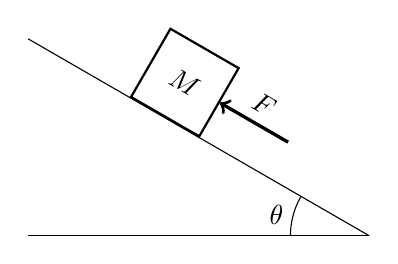
\begin{tikzpicture}
        %% Surface
        \draw (0,0) -- (150:5);
        \draw (0,0) -- (180:4.33);
        %% block
        \node[draw,thick,anchor=south,rotate=-30,minimum size=1cm] (M) at (150:3) {$M$};
        \draw[very thick,<-] (M.east) -- ++(-30:1) node[pos=0.5,anchor=south,rotate=-30] {$F$};
        %% angle
        \draw (-1,0) arc (180:150:1) node[pos=0.5,anchor=east] {$\theta$};
    \end{tikzpicture}
    \end{center}
    The block moves up the incline at a constant velocity of \SI{5}{\meter\per\second}.
    What is the power required accomplish this situation?
    \begin{multicols}{2}
    \begin{choices}
        \wrongchoice{$5F\cos\theta$}
        \wrongchoice{$F\cos\theta$}
      \correctchoice{$5Mg\sin\theta$}
        \wrongchoice{$5Mg\cos\theta$}
        \wrongchoice{$F\sin\theta$}
    \end{choices}
    \end{multicols}
\end{question}
}

\element{ap}{
\begin{question}{power-q03}
    In the diagram,
        a box of mass $m$ is sliding down a frictionless ramp of length $L$ with an incline of $\theta$ to the horizontal.
    The mass takes $t$ seconds to slide down the ramp.
    \begin{center}
    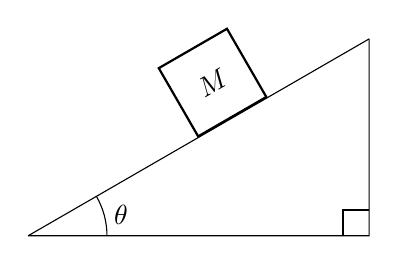
\begin{tikzpicture}
        %% Surface
        \draw (0,0) -- (30:5);
        \draw (0,0) -- (4.33,0) -- (30:5);
        \draw[thick] (4,0) -- (4,0.33) -- (4.33,0.33);
        %% block
        \node[draw,thick,anchor=south,rotate=30,minimum size=1cm] (M) at (30:3) {$M$};
        %% angle
        \draw (1,0) arc (0:30:1) node[pos=0.5,anchor=west] {$\theta$};
    \end{tikzpicture}
    \end{center}
    The power exerted by gravity during the slide is:
    \begin{multicols}{2}
    \begin{choices}
        \wrongchoice{$\dfrac{mg\sin\theta}{t}$}
        \wrongchoice{$mgt\cos\theta$}
        \wrongchoice{$mgt\sin\theta$}
      \correctchoice{$\dfrac{mgL\sin\theta}{t}$}
        \wrongchoice{$\dfrac{mgL\cos\theta}{t}$}
    \end{choices}
    \end{multicols}
\end{question}
}

\element{ap}{
\begin{question}{power-q04}
    A crate with mass \SI{40}{\kilo\gram} is pulled by a worker along a surface at a constant velocity for \SI{10}{\meter}.
    If the crate is pulled for \SI{5}{\second},
        and the coefficient of kinetic friction between the surface and the crate is \num{0.5},
        the power exerted by the worker over this time is most nearly:
    \begin{multicols}{3}
    \begin{choices}
        \wrongchoice{\SI{20}{\watt}}
        \wrongchoice{\SI{40}{\watt}}
        \wrongchoice{\SI{100}{\watt}}
        \wrongchoice{\SI{200}{\watt}}
      \correctchoice{\SI{400}{\watt}}
    \end{choices}
    \end{multicols}
\end{question}
}

\element{ap}{
\begin{question}{power-q05}
    Of the following, which is \emph{not} a unit of power?
    \begin{choices}
        \wrongchoice{Watt (\si{\watt})}
        \wrongchoice{Joule per second (\si{\joule\per\second})}
        \wrongchoice{Kilogram meter squared per second cubed (\si{\kilo\gram\meter\squared\per\second\cubed})}
      \correctchoice{Kilowatt hour (\si{\kilo\watt\hour})}
        \wrongchoice{Ampere volt (\si{\ampere\volt})}
    \end{choices}
\end{question}
}

\element{ap}{
\begin{question}{power-q06}
    A person pushes an object with a mass of \SI{50}{\kilo\gram} across a surface with a coefficient of friction of \num{0.2}.
    If the box moves with a constant velocity of \SI{2.0}{\meter\per\second},
        the power supplied to the box by the person is:
    \begin{multicols}{3}
    \begin{choices}
        \wrongchoice{\SI{20}{\watt}}
        \wrongchoice{\SI{25}{\watt}}
        \wrongchoice{\SI{50}{\watt}}
        \wrongchoice{\SI{100}{\watt}}
      \correctchoice{\SI{200}{\watt}}
    \end{choices}
    \end{multicols}
\end{question}
}

\element{ap}{
\begin{question}{power-q07}
    How much power is needed to lift a \SI{100}{\kilo\gram} block vertically upward at a constant speed of \SI{5}{\meter\per\second}?
    \begin{multicols}{2}
    \begin{choices}
        \wrongchoice{\SI{2 500}{\watt}}
      \correctchoice{\SI{5 000}{\watt}}
        \wrongchoice{\SI{7 500}{\watt}}
        \wrongchoice{\SI{10 000}{\watt}}
        \wrongchoice{\SI{0}{\watt} because the object is at a constant velocity}
    \end{choices}
    \end{multicols}
\end{question}
}

\element{ap}{
\begin{question}{power-q08}
    A crane lifts a box upward that weighs \SI{2000}{\newton} at a constant speed of \SI{8}{\meter\per\second}.
    What is the power input of the crane to lift the box?
    \begin{multicols}{2}
    \begin{choices}
        \wrongchoice{\SI{250}{\watt}}
        \wrongchoice{\SI{1 250}{\watt}}
        \wrongchoice{\SI{8 000}{\watt}}
      \correctchoice{\SI{16 000}{\watt}}
        \wrongchoice{\SI{32 000}{\watt}}
    \end{choices}
    \end{multicols}
\end{question}
}

\element{ap}{
\begin{question}{power-q09}
    A helicopter lifts a large crate weighing \SI{4000}{\newton} expending a constant power of \SI{8}{\kilo\watt}.
    The crate is moving upward at a constant velocity of:
    \begin{multicols}{3}
    \begin{choices}
      \correctchoice{\SI{2}{\meter\per\second}}
        \wrongchoice{\SI{4}{\meter\per\second}}
        \wrongchoice{\SI{8}{\meter\per\second}}
        \wrongchoice{\SI{16}{\meter\per\second}}
        \wrongchoice{\SI{50}{\meter\per\second}}
    \end{choices}
    \end{multicols}
\end{question}
}

\element{ap}{
\begin{question}{power-q10}
    A \SI{300}{\newton} object is lifted \SI{10}{\meter} by a crane at a constant rate in \SI{15}{\second}.
    The average power expended to lift the object is:
    \begin{multicols}{2}
    \begin{choices}
        \wrongchoice{\SI{2}{\watt}}
        \wrongchoice{\SI{20}{\watt}}
        \wrongchoice{\SI{200}{\watt}}
      \correctchoice{\SI{2 000}{\watt}}
        \wrongchoice{\SI{20 000}{\watt}}
    \end{choices}
    \end{multicols}
\end{question}
}

\element{ap}{
\begin{question}{power-q11}
    A \SI{500}{\newton} student expends an average power of \SI{250}{\watt} to climb a 6 m vertical rope at constant velocity.
    How long does it take for the student to climb the rope?
    \begin{multicols}{3}
    \begin{choices}
        \wrongchoice{\SI{1}{\second}}
        \wrongchoice{\SI{2}{\second}}
        \wrongchoice{\SI{3}{\second}}
        \wrongchoice{\SI{6}{\second}}
      \correctchoice{\SI{12}{\second}}
    \end{choices}
    \end{multicols}
\end{question}
}

\element{ap}{
\begin{question}{power-q12}
    The work done by an object is given by the equation $W(t) = 3t^2 - 5t + 1$,
        where $W$ is in joules and $t$ is in seconds.
    What is the power delivered by the object at $t=2$?
    \begin{multicols}{3}
    \begin{choices}
        \wrongchoice{\SI{3}{\watt}}
        \wrongchoice{\SI{6}{\watt}}
      \correctchoice{\SI{7}{\watt}}
        \wrongchoice{\SI{8}{\watt}}
        \wrongchoice{\SI{10}{\watt}}
    \end{choices}
    \end{multicols}
\end{question}
}

\element{ap}{
\begin{question}{power-q13}
    The power delivered by an object is given by the equation $P(t) = 6t - 3$,
        where $P$ is in watts and $t$ is in seconds.
    How much work is done by the object during the interval $0<t<\SI{4}{\second}$?
    \begin{multicols}{3}
    \begin{choices}
        \wrongchoice{\SI{16}{\joule}}
        \wrongchoice{\SI{21}{\joule}}
        \wrongchoice{\SI{24}{\joule}}
      \correctchoice{\SI{36}{\joule}}
        \wrongchoice{\SI{48}{\joule}}
    \end{choices}
    \end{multicols}
\end{question}
}

\element{ap}{
\begin{question}{power-q14}
    The position of an object is given by the equation $x(t) = t^2 + 3t + 4$,
        where $x$ is in meters and $t$ is in seconds.
    A constant force of \SI{10}{\newton} acts on the object.
    What is the power delivered to the object at $t=\SI{5}{\second}$?
    \begin{multicols}{3}
    \begin{choices}
        \wrongchoice{\SI{100}{\watt}}
        \wrongchoice{\SI{104}{\watt}}
      \correctchoice{\SI{130}{\watt}}
        \wrongchoice{\SI{134}{\watt}}
        \wrongchoice{\SI{200}{\watt}}
    \end{choices}
    \end{multicols}
\end{question}
}

\element{ap}{
\begin{question}{power-q15}
    The velocity of an object is given by the equation $v(t) = 2t + 5$,
        where $v$ is in meters per second and $t$ is in seconds.
    A constant force of \SI{6}{\newton} acts on the object.
    What is the power delivered to the object at $t=\SI{3}{\second}$?
    \begin{multicols}{3}
    \begin{choices}
        \wrongchoice{\SI{55}{\watt}}
        \wrongchoice{\SI{61}{\watt}}
      \correctchoice{\SI{66}{\watt}}
        \wrongchoice{\SI{71}{\watt}}
        \wrongchoice{\SI{77}{\watt}}
    \end{choices}
    \end{multicols}
\end{question}
}

\element{ap}{
\begin{question}{power-q16}
    The acceleration of an object is given by the equation $a(t)=2$,
        where $a$ is in meter per second squared and $t$ is in seconds.
    The object is initially at rest at the origin.
    A constant force of \SI{30}{\newton} acts on the object.
    What is the power delivered to the object at $t=\SI{9}{\second}$?
    \begin{multicols}{3}
    \begin{choices}
        \wrongchoice{\SI{240}{\watt}}
        \wrongchoice{\SI{360}{\watt}}
      \correctchoice{\SI{540}{\watt}}
        \wrongchoice{\SI{600}{\watt}}
        \wrongchoice{\SI{810}{\watt}}
    \end{choices}
    \end{multicols}
\end{question}
}

\element{ap}{
\begin{question}{power-q17}
    The power delivered to an object at $t=\SI{2}{\second}$ is \SI{170}{\watt}.
    The position of the object along the $x$-axis is given by the equation $x(t)=3t^2+5t+1$,
        where $x$ is in meters and $t$ is in seconds.
    Which of the following is closest to the force acting on the object?
    \begin{multicols}{3}
    \begin{choices}
        \wrongchoice{\SI{8}{\newton}}
        \wrongchoice{\SI{9}{\newton}}
      \correctchoice{\SI{10}{\newton}}
        \wrongchoice{\SI{11}{\newton}}
        \wrongchoice{\SI{12}{\newton}}
    \end{choices}
    \end{multicols}
\end{question}
}

\element{ap}{
\begin{question}{power-q18}
    If a mass of \SI{10}{\kilo\gram} moves with the velocity $v(t)=t^2-2t+1$,
        where $v$ is in meters per second and $t$ is in seconds,
        What is the power exerted by the force pushing the mass at $t=\SI{2}{\second}$?
    \begin{multicols}{3}
    \begin{choices}
        \wrongchoice{\SI{5}{\watt}}
        \wrongchoice{\SI{10}{\watt}}
      \correctchoice{\SI{20}{\watt}}
        \wrongchoice{\SI{30}{\watt}}
        \wrongchoice{\SI{50}{\watt}}
    \end{choices}
    \end{multicols}
\end{question}
}


\endinput


